\chapter{Spécification fonctionnelle}

\section{Les tâches principales}

\subsection{Se déplacer}

Le déplacement est bien entendu un élément cruciale de la conception
d'un robot. La desserte robotisée a ceci de particulier qu'elle doit
évoluer en milieu humain. Cela demande de définir exactement quand le
robot est en risque de rencontrer des humains, et comment il doit
réagir.

Au dela de cet aspect, nous devons également définir tous les types de
déplacements que le robot devra effectuer:

\begin{itemize}
\item Construction de carte
\item arrivée en salle
\item déambulation
\item gestion de groupe
\item suivi
\item dirigé
\item retour à la base
\item utilisation de l'interface
\end{itemize}

\subsubsection{Mode construction de carte}
La construction de carte est l'action primaire du robot lui permettant par la suite de se repérer dans la salle. C'est pourquoi elle doit se dérouler avant l'arrivée des convives ou après leur départ. C'est durant cette phase que le robot crée un carte de la salle de cocktail dans laquelle il va devoir se déplacer. Ainsi, lors de la réception, il pourra savoir se positionner dans la salle de réception.

La phase de construction de carte se déclenche par un élément externe comme le maître de réception. Pour déclencher se mode il faut que le robot soit dans la salle à cartographier. C'est à dire que le robot peut y être présent avant le lancement d'un autre mode de déplacement ou après avoir suivi la personne qui enclenchera le mode, soit après le mode suivi.

la cartographie se réalise à l'aide de deux caméra. Le robot se déplace seulement pour peaufiner sa carte. Sinon le robot tourne sur lui-même pour réaliser sa carte de repère. Ce mode se termine lorsque le robot a réalisé sa carte. 

Après avoir enclenché réalisé la carte, le robot devra rentrer à sa base avant le lancement de la soirée cocktail.

Les points d'entrées du mode sont:
\begin{itemize}
\item aucun mode
\item Le mode suivi
\end{itemize}

Les points de sorties du mode sont:
\begin{itemize}
\item le mode retour à la base.
\end{itemize}

\subsubsection{Mode arrivée en salle}

Le déplacement de la base vers la salle est la première chose que doit réaliser 
le robot avant de commencer sa déambulation. C’est donc  le moment où il vérifie 
que ses batteries sont chargées, que son plateau est rempli et qu’il connait le 
chemin vers la salle. Le mouvement de la base vers la salle peut être déjà cartographié.
Cet évènement ne peut arriver que s’il est déjà à sa base.

Les points d'entrées du mode sont:
\begin{itemize}
\item Le mode retour à la base
\item Le mode dirigé
\item Le mode suivi
\end{itemize}

Les points de sorties du mode sont:
\begin{itemize}
\item le mode déhambulation.
\end{itemize}


\subsubsection{Mode déambulation}

Le mode déambulation est l'un des princpaux mode de déplacement de la
desserte. Il s'agit pour le robot de repérer un groupe de convive puis
de se déplacer vers lui. Un des point clé de ce déplacement est que le
robot doit éviter de retourner sur une zone géographique qu'il à déjà
servi.

le déroulement du mode se fait comme suit:
\begin{itemize}
\item déclenchement du mode à l'arrivée dans la salle.
\item la disserte va de groupe en groupe et le cas échéant de table en
  table.
\item le robot garde en mémoire les zones géographiques déjà
  desservies et priorise les zones encore non servie.
\item Fin du mode de déambulation à la fin d'un timer et/ou après une
  diminution significative du poids du plateau, ou en cas d'absence
  d'espace ou passer (interieur d'un groupe), ou en cas de rencontre
  d'un groupe.\\
\end{itemize}

les points d'entrée du mode sont:
\begin{itemize}
\item le mode utilsation de l'interface
\item le mode arrivée en salle
\item le mode suivi
\item le mode dirigé\\
\end{itemize}

les points de sorties du mode sont:
\begin{itemize}
\item le mode suivi
\item le mode dirigé
\item le mode retour à la base
\item le mode gestion de groupe
\item le mode utilisation de l'interface\\
\end{itemize}

\subsubsection{Mode gestion de groupe}

\subsubsection{Mode suivi}

\subsubsection{Mode dirigé}

\subsubsection{Mode retour a la base}

Ce mode permet au robot de rentrer à la base lorsqu'il en a besoin
(ravitaillement, disfonctionnement, rappel du maitre d'hotel...).

le déroulement du mode se fait comme suit:
\begin{itemize}
\item déclenchement lorsque le plateau est vide et/ou timer, en cas de
  detection d'anomalie, ou de rappel à la base.
\item en cas de déplacement impossible, envoie une demande demande
  d'assistance.
\item cherche le plus court chemin ne passant pas par des groupes
\item fin du mode lorsque le robot arrive à la base.\\
\end{itemize}

les points d'entrée du mode sont:
\begin{itemize}
\item le mode déambulation
\item le mode utilsation de l'interface
\item le mode arrivée en salle
\item le mode suivi
\item le mode dirigé\\
\end{itemize}

les points de sorties du mode sont:
\begin{itemize}
\item le mode suivi
\item le mode dirigé
\item le mode utilisation de l'interface\\
\end{itemize}

\subsubsection{Mode utilisation interface}
Le robot entre dans ce mode lorsque quelqu'un utilise une des
interfaces du robot. Dans ce cas le robot doit cesser de se deplacer.

\subsection{schéma générale}

\begin{figure}[h]
\begin{center}
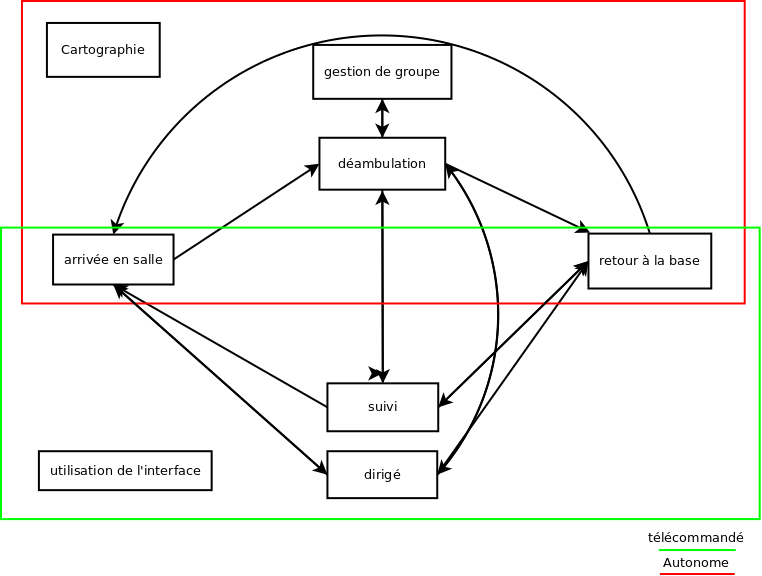
\includegraphics[scale=0.55]{Images/transition_mode.png}
\caption{Transition des modes}
\label{Transition des modes}
\end{center}
\end{figure}

\subsection{Servir}

\subsubsection{Maintenir le plateau}

\subsubsection{Presenter le plateau}

\subsection{Communication}
 
